\documentclass[xcolor={svgnames},
               hyperref={colorlinks,citecolor=DeepPink4,linkcolor=FireBrick,urlcolor=Maroon}]
               {beamer}

\mode<presentation>{
  \usetheme{Madrid}
  \usecolortheme{seagull}
  \setbeamercovered{transparent}
  \setbeamerfont{frametitle}{size=\large}
}

\setbeamercolor*{block title}{bg=red!10}
\setbeamercolor*{block body}{bg=red!5}

\usepackage[english]{babel}
\usepackage[latin1]{inputenc}
\usepackage{times}
\usepackage[T1]{fontenc}
% Or whatever. Note that the encoding and the font should match. If T1
% does not look nice, try deleting the line with the fontenc.

\usepackage{empheq,bm}
\usepackage{xspace}
\usepackage{fancyvrb}

\usepackage{tikz}
\usetikzlibrary{shapes,arrows.meta,decorations.markings,decorations.pathreplacing,fadings,positioning}

\usepackage[kw]{pseudo}
\pseudoset{left-margin=15mm,topsep=5mm,idfont=\texttt,st-left=,st-right=}


% If you wish to uncover everything in a step-wise fashion, uncomment
% the following command:
%\beamerdefaultoverlayspecification{<+->}

\newcommand{\ba}{\mathbf{a}}
\newcommand{\bb}{\mathbf{b}}
\newcommand{\bc}{\mathbf{c}}
\newcommand{\bbf}{\mathbf{f}}
\newcommand{\bg}{\mathbf{g}}
\newcommand{\bn}{\mathbf{n}}
\newcommand{\bq}{\mathbf{q}}
\newcommand{\br}{\mathbf{r}}
\newcommand{\bx}{\mathbf{x}}
\newcommand{\by}{\mathbf{y}}
\newcommand{\bv}{\mathbf{v}}
\newcommand{\bu}{\mathbf{u}}
\newcommand{\bw}{\mathbf{w}}

\newcommand{\bF}{\mathbf{F}}
\newcommand{\bG}{\mathbf{G}}
\newcommand{\bQ}{\mathbf{Q}}

\newcommand{\grad}{\nabla}
\newcommand{\Div}{\nabla\cdot}

\newcommand{\argmin}{\operatorname{argmin}}

\newcommand{\CC}{\mathbb{C}}
\newcommand{\EE}{\mathbb{E}}
\newcommand{\RR}{\mathbb{R}}

\newcommand{\ddt}[1]{\ensuremath{\frac{\partial #1}{\partial t}}}
\newcommand{\ddx}[1]{\ensuremath{\frac{\partial #1}{\partial x}}}
\newcommand{\Matlab}{\textsc{Matlab}\xspace}
\newcommand{\Octave}{\textsc{Octave}\xspace}
\newcommand{\eps}{\epsilon}

\newcommand{\ip}[2]{\left<#1,#2\right>}

\newcommand{\xiphalf}{{x_{i+\frac{1}{2}}}}
\newcommand{\ximhalf}{{x_{i-\frac{1}{2}}}}
\newcommand{\Fiphalf}{{F_{i+\frac{1}{2}}}}
\newcommand{\Fimhalf}{{F_{i-\frac{1}{2}}}}
\newcommand{\Fiphalfn}{{F^n_{i+\frac{1}{2}}}}
\newcommand{\Fimhalfn}{{F^n_{i-\frac{1}{2}}}}

\newcommand{\trefcolumn}[1]{\begin{bmatrix} \phantom{x} \\ #1 \\ \phantom{x} \end{bmatrix}}
\newcommand{\trefmatrixtwo}[2]{\left[\begin{array}{c|c|c} & & \\ #1 & \dots & #2 \\ & & \end{array}\right]}
\newcommand{\trefmatrixthree}[3]{\left[\begin{array}{c|c|c|c} & & & \\ #1 & #2 & \dots & #3 \\ & & & \end{array}\right]}
\newcommand{\trefmatrixgroups}[4]{\left[\begin{array}{c|c|c|c|c|c} & & & & & \\ #1 & \dots & #2 & #3 & \dots & #4 \\ & & & & & \end{array}\right]}

\newcommand{\blocktwo}[4]{\left[\begin{array}{c|c} #1 & #2 \\ \hline #3 & #4 \end{array}\right]}

\newcommand{\bqed}{{\color{blue}\qed}}
\newcommand{\ds}{\displaystyle}

\newcommand\mynum[1]{{\renewcommand{\insertenumlabel}{#1}%
      \usebeamertemplate{enumerate item} \,}}


\title{Online optimization}

\subtitle{\emph{ML training algorithms reduce regret}}

\author{Ed Bueler}

\institute[UAF]{MATH 692 Mathematics for Machine Learning}

\date[Spring 2022]{17 March}

%\titlegraphic{\begin{picture}(0,0)
%    \put(0,180){\makebox(0,0)[rt]{\includegraphics[width=4cm]{figs/software.png}}}
%  \end{picture}
%}

%% to start section counter at 0 see
%% https://tex.stackexchange.com/questions/170222/change-the-numbering-in-beamers-table-of-content


\begin{document}
\beamertemplatenavigationsymbolsempty

\begin{frame}
  \maketitle
\end{frame}


\begin{frame}{Outline}
  \tableofcontents[hideallsubsections]
\end{frame}


\begin{frame}{my motivations}

\begin{itemize}
\item why is SGD so popular? is my algorithm better than yours?

\medskip
\item it was easy to stumble upon:

\medskip
\begin{center}
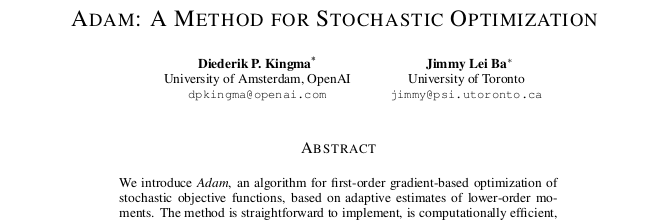
\includegraphics[width=0.7\textwidth]{figs/adam-paper.png}
\end{center}

\medskip
    \begin{itemize}
    \item[$-$] 100651 citations
    \item[$-$] the Adam optimizer is the default for \href{https://www.tensorflow.org/tutorials/keras/classification}{tensorflow}, \href{https://pytorch.org/docs/stable/optim.html}{pytorch}, \dots
    \end{itemize}

\medskip
\item so, how do they analyze Adam and show that it is good?
    \begin{itemize}
    \item[] \emph{answer}: this talk
    \end{itemize}
\end{itemize}
\end{frame}


\section{online optimization framework}

\begin{frame}{training a neural net ($=$ recalling my earlier talk)}

\begin{itemize}
\item forward pass through an artificial neural net (ANN) with $L$ layers:

\begin{columns}
\begin{column}{0.1\textwidth}
$x^{\{i\}}\to$ 
\end{column}
\begin{column}{0.4\textwidth}
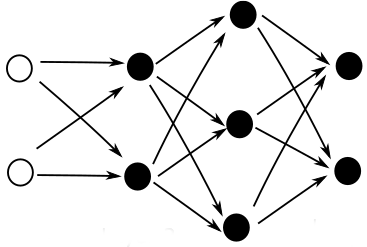
\includegraphics[height=30mm]{figs/cleannet.png}
\end{column}
\begin{column}{0.45\textwidth}
$\to a^{[L]}$ \hfill (supposed to be $y^{\{i\}}$)
\end{column}
\end{columns}

\item output activations are a function of input and parameters:
    $$a^{[L]} = a^{[L]}(x^{\{i\}}; p)$$
\item parameters $p$ collect weights and biases:
    $$p=\{W^{[2]},\dots,W^{[L]},b^{[2]},\dots,b^{[L]}\} \in \RR^n$$
\item cost of one labeled pair $(x^{\{i\}},y^{\{i\}})$:
    $$C^{\{i\}}(p) = \frac{1}{2} \left\|y^{\{i\}} - a^{[L]}(x^{\{i\}}; p)\right\|_2^2$$
\end{itemize}
\end{frame}


\begin{frame}{notation (standardization and simplification)}

\begin{itemize}
\item $\theta = p$ is vector of parameters
\item $(x_i,y_i) = (x^{\{i\}},y^{\{i\}})$ is a labeled pair
\item $N$ is total size of training set
\item $c_i(\theta) = \frac{1}{2} \left\|y_i - a^{[L]}(x_i; \theta)\right\|_2^2 = C^{\{i\}}(p)$ is cost of one pair
\end{itemize}
\end{frame}


\begin{frame}{total cost versus online cost sequence}

\begin{block}{total cost of training set}
\textbf{original goal:}  minimize total (average) cost over fixed training set
    $$\frac{1}{N} \sum_{i=1}^N c_i(\theta)$$
\end{block}

\begin{block}{online training $=$ sequence of cost objectives}
assume infinite sequence of cost functionals:
    $$c_i(\theta)$$
\end{block}

\begin{itemize}
\item the basic online training \textbf{method} is clear: train the neural net incrementally, a little for each $c_i$
\item \textbf{but what's the new online goal?}
\end{itemize}

\end{frame}


\begin{frame}{online training algorithms}

\begin{itemize}
\item somehow choose $\theta_1$ as the initial iterate for the parameters
\item an \emph{online training algorithm} computes each new iterate $\theta_{i+1}$
\item $\theta_{i+1}$ is computed from previous cost functionals $\{c_1,c_2,\dots,c_i\}$ and (parameter) iterates $\{\theta_1,\theta_2,\dots,\theta_i\}$
\item \textbf{key assumption:} an online  training algorithm does not use \emph{future} cost functionals in constructing $\theta_{i+1}$:
    $$\theta_{i+1} = F(c_1,\dots,c_i,\theta_1,\dots,\theta_i)$$
\end{itemize}
\end{frame}


\begin{frame}{online training algorithm examples}

\begin{itemize}
\item ``stochastic'' gradient descent with varying learning rates $\eta_i$:
   $$\theta_{j+1} = \theta_i - \eta_i \grad c_i(\theta_i)$$

    \begin{itemize}
    \item[$\circ$] called \emph{online gradient descent} (OGD) from now on
    \item[$\circ$] probability is not needed!
    \end{itemize}
\item Adam (\emph{more later})
\item Adaline, Adadelta, Adagrad, RMSprop, mini-batching, dropout, \dots
    \begin{itemize}
    \item[$\circ$] google search for buzzwords: \quad \texttt{tensorflow optimizers}
    \end{itemize}
\item (quasi-)Newton methods which use (approximate) 2nd derivatives
\end{itemize}
\end{frame}


\section{regret}

\begin{frame}{regret of an online algorithm}

\begin{block}{\textbf{definition} (Zinkevich, 2003; decision theory in 1980s?)}
the \emph{regret} of an online algorithm, at the $k$th training step, is
    $$R_k = \sum_{i=1}^k c_i(\theta_i) - \min_\theta \sum_{i=1}^k c_i(\theta)$$
\end{block}

\begin{itemize}
\item regret $R_k$ is the difference between the algorithm result for the stream so far $\{c_1,\dots,c_k\}$ and the best-possible cost from a single parameter setting
    \begin{itemize}
    \item[$\circ$] best setting so far:\quad  $\ds \theta_k^* = \begin{smallmatrix} \phantom{x} \\ \text{\footnotesize argmin} \\ \theta \end{smallmatrix} \sum_{i=1}^k c_i(\theta)$
    \end{itemize}

\smallskip
\item $R_k>0$: the player regrets not choosing $\theta_k^*$
\item negative regret is possible!
\end{itemize}
\end{frame}


\begin{frame}{regret in game theory}

\begin{itemize}
\item treat the algorithm as a \emph{player} and the online stream of cost functionals $c_i$ as an \emph{adversary}
\item the player chooses $\theta_{i+1}$ \underline{before} knowing $c_{i+1}$
\item the adversarial sequence $\{c_i\}$ is totally uncontrolled
\end{itemize}

\begin{block}{online convex game (Abernathy et al 2008)}
\begin{pseudo*}
for $i = 0,1,\dots,k-1$ \\+
    \st{player chooses} $\theta_{i+1}$ \\
    \st{adversary chooses} $c_{i+1}$ \\-
\st{player suffers regret} \\+
    $\ds R_k = \sum_{i=1}^k c_i(\theta_i) - \min_\theta \sum_{i=1}^k c_i(\theta)$
\end{pseudo*}
\end{block}
\end{frame}


\begin{frame}{convex sets}

\begin{itemize}
\item previous slide says ``convex''; we need the definition
\end{itemize}

\begin{block}{definition}
\begin{itemize}
\item a set $K \subset \RR^n$ is \emph{convex} if for all $x,y \in K$ and $0 \le t \le 1$,
  $$t\, x + (1-t) y \in K$$

    \begin{itemize}
    \item[$\circ$] line segment from
    \item[]  $x$ to $y$ is inside $K$
    \end{itemize}

\vspace{-8mm}
\hfill 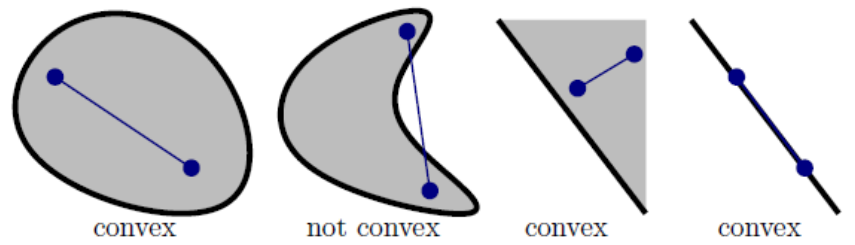
\includegraphics[width=0.6\textwidth]{figs/convex}
\end{itemize}
\end{block}
\end{frame}


\begin{frame}{convex functions}

\begin{itemize}
\item convex sets \emph{and} functions
\end{itemize}

\begin{block}{definition}
\begin{itemize}
\item a function $f:K \to \RR$ is \emph{convex} if for all $x,y \in K$ and $0 \le t \le 1$,
  $$t\, f(x) + (1-t) f(y) \ge f(t\, x + (1-t) y)$$
\end{itemize}
\end{block}

\begin{itemize}
\item for $f:K\to \RR$ to be convex, note $K$ must be convex
\item convex = concave \emph{up}
\end{itemize}
\end{frame}


\begin{frame}{convex optimization: a classical topic}

\begin{block}{definition}
given a convex set $K \subset \RR^n$ and a convex function $f:K\to \RR$, we say that the problem
    $$\min_{\theta \in K} f(\theta)$$
is a \emph{convex optimization problem}
\end{block}

\begin{itemize}
\item $K$ is often described by equality and inequality constraints
\item $K=\RR^n$ is convex (unconstrained optimization)
\item SVM is convex optimization, with nontrivial $K$
\item \emph{I don't know the answer}:

for an ANN, when is $C^{\{i\}}(p) = \frac{1}{2} \left\|y^{\{i\}} - a^{[L]}(x^{\{i\}}; p)\right\|_2^2$ a convex function on $K = \RR^n$?
\end{itemize}
\end{frame}


\begin{frame}{convex optimization: the default algorithm}

\begin{itemize}
\item to solve $\ds \min_{\theta \in K} f(\theta)$
\item assume $K\subset \RR^n$ is closed and convex
\item assume $f$ is differentiable (\emph{and convex if you are optimistic})
\item assume learning rates (\emph{step sizes}) $\eta_i>0$
\end{itemize}

\begin{block}{projected gradient descent}

\begin{pseudo*}
\st{choose} $\theta_1 \in K$ \\
for $i = 1,2,\dots$ \\+
    $\theta_{i+1} = \Pi_K \big(\theta_i - \eta_i \grad f(\theta_i)\big)$
\end{pseudo*}
\end{block}

\begin{itemize}
\item each $y\in \RR^n$ has a unique \emph{projection} $w = \Pi_K(y) \in K$ so that
    $$w = \argmin_x \|y - x\|_2$$

    \begin{itemize}
    \item[$-$] $\Pi_K(y)$ is the closest point in $K$ to $y$
    \end{itemize}
\end{itemize}
\end{frame}


\begin{frame}{online convex optimization}

\begin{itemize}
\item convex optimization is \emph{so}\, 20th century \dots let's go online!
\end{itemize}

\begin{block}{definition}
\emph{online convex optimization}:

\begin{itemize}
\item fix a convex set $K\subset \RR^n$
\item assume a sequence of convex functions $c_i:K\to \RR$
\item choose an algorithm for generating $\theta_{i+1} \in K$ from previous $c_i$
\end{itemize}
\end{block}

\begin{itemize}
\item online convex optimization = online convex programming
\item this is \emph{not} a stochastic problem
\item online gradient descent (OGD) is projected gradient descent with changing $f=c_i$:
    $$\theta_{i+1} = \Pi_K \big(\theta_i - \eta_i \grad c_i(\theta_i)\big)$$
\item the goal of any online algorithm is to \textbf{not suffer big regret}
\end{itemize}
\end{frame}


\begin{frame}{regarding regret: quotes from Zinkevich (2003)}

\emph{We make \textbf{no distributional assumptions} about the convex cost functions.}

\medskip
\noindent \emph{We cannot hope to choose a point $\theta_i$ that minimizes $c_i$, because $c_i$ can be anything. Instead we try to minimize regret.}

\medskip
\noindent \emph{If the sequence of cost functions $\{c_i\}$ is relatively stationary, then an online algorithm can learn what the cost functions will look like in the future.  If the sequence of cost functions varies drastically, then the offline algorithm will not be able to take advantage of this because it selects a single $\theta$.}

  $$R_k = \underbrace{\sum_{i=1}^k c_i(\theta_i)}_{\text{online alg.~result}} - \,\, \underbrace{\min_\theta \sum_{i=1}^k c_i(\theta)}_{\text{offline result}}$$
\end{frame}


\begin{frame}{how big is your regret?}

\begin{itemize}
\item the online optimization framework evaluates an ML training algorithm via a \emph{regret bound}:
    \begin{itemize}
    \item[$-$] does $R_k$ grow or decay with $k$?
    \item[$-$] how fast does it grow?
    \item[$-$] what properties of the objectives $c_i$ determine the bound?
    \item[$-$] what algorithmic settings determine the bound?
    \end{itemize}
\item actually online (= fed by internet) ML training might not want the ``best'' offline setting \quad $\theta_k^* = \begin{smallmatrix} \phantom{x} \\ \text{\footnotesize argmin} \\ \theta \end{smallmatrix} \sum_{i=1}^k c_i(\theta)$, \, even if it is attainable
\end{itemize}
\end{frame}


\section{analysis of online gradient descent (OGD)}

\begin{frame}{Hazan bound}

\begin{itemize}
\item we need an example of a bound
\item first bound for OGD assumes nice costs $c_i$
\end{itemize}

\begin{block}{theorem (Hazan et al., 2007)}
Suppose the $c_i$ are uniformly strictly convex: $\grad^2 c_i \succ H > 0$.  Suppose we run OGD to find iterates $\theta_1,\dots,\theta_k$.  Let $G = \max_{i=1,\dots,k} \|\grad c_i(\theta_i)\|$.  Then
    $$R_k \le \frac{G^2}{2 H} (1 + \log k)$$
\end{block}
\end{frame}


\begin{frame}{x}

\begin{itemize}
\item fixme
\end{itemize}
\end{frame}


\begin{frame}{OGD average regret goes to zero}

\begin{itemize}
\item STATE COROLLARY
\item this is the closest I've come to understanding why OGD (SGD) is a ``good'' algorithm for ML training
\end{itemize}
\end{frame}


\begin{frame}{other algorithms}

\begin{itemize}
\item follow the leader
\item Newton
\item quasi-Newton
\end{itemize}
\end{frame}


\section{Adam's regret}

\begin{frame}{fixme}

\begin{itemize}
\item fixme
\end{itemize}
\end{frame}


\section{frameworks, including empirical risk}

\begin{frame}{risk and empirical risk}

\begin{itemize}
\item the \emph{Deep Learning} book (Chapter 8), for example, tells you that ML optimization is special because the data is stochastic

\begin{block}{definition}
the \emph{risk} of an ANN parameter setting is the expected cost over an assumed  training data distribution
\end{block}

    \begin{itemize}
    \item[$-$] typically assumes each $(x_i,y_i)$ is an independent sample
    \end{itemize}

\item but you don't tend to know the distribution, so \dots

\begin{block}{definition}
the \emph{empirical risk} of an ANN parameter setting is the average cost over the training data set
\end{block}

    \begin{itemize}
    \item[$-$] this is really the same as \emph{maximum likelihood estimation}
    \end{itemize}

\end{itemize}
\end{frame}


\begin{frame}{the 5 frameworks for ML training optimization}

\begin{itemize}
\item it seems ML optimization is portrayed in 5 different ways:

\medskip
    \begin{enumerate}
    \item[1.] \textbf{risk} = find parameters which minimize expected cost over assumed distribution for training data
    \item[2.] \textbf{empirical risk} = find parameters which minimize sample mean over training data
    \item[3.] \textbf{maximum likelihood estimation} = find parameters which maximize assumed distribution form (e.g.~exp of negative cost)
    \item[4.] naive \textbf{optimization} = find parameters which minimize average or sum of costs of training data
    \item[5.] \textbf{online regret} = an algorithm generating $\theta_{i+1}$ from previous $c_i$ should have small regret
    \end{enumerate}

\bigskip
\item 1 is only notional
    \begin{itemize}
    \item[$-$] the training data distribution is unknown
    \end{itemize}
\item 2,3,4 are the same goal once you remove probabilistic edifice
\item only 5 aligns with the \emph{algorithm designer's} concerns
    \begin{itemize}
    \item[$-$] 5 is \emph{meta-} ML training optimization
    \end{itemize}
\end{itemize}
\end{frame}


\begin{frame}{the 5 frameworks: formulas}

\begin{enumerate}
\item[1.] \textbf{risk}:
    $$\min_\theta \EE[c(\theta)] = \min_\theta \int_{\{\text{all } (x,y)\}} c(\theta;x,y)\,dp_{\text{data}}$$
\item[2.] \textbf{empirical risk}
\item[3.] = \textbf{maximum likelihood estimation}
\item[4.] = \textbf{optimization}:
    $$\min_\theta \frac{1}{k} \sum_{i=1}^k c_i(\theta)$$
\item[5.] \textbf{online regret}:
    $$\min_{\text{alg.~for } \theta_{i+1}} \left[\sum_{i=1}^k c_i(\theta_i) - \min_\theta \sum_{i=1}^k c_i(\theta)\right]$$
\end{enumerate}
\end{frame}


\begin{frame}{why online regret bounds?}

\begin{itemize}
\item by proving an online regret bound you identify a rigorous property of the minimization algorithm
\item quantitative regret bounds distinguish between:
    \begin{itemize}
    \item[$-$] different algorithms (\textbf{ex.}~OGD versus Adam, $\eta_i$ choices, \dots)
    \item[$-$] different cost functions (convex versus strictly convex)
    \end{itemize}
\item analysis of regret bypasses probabilistic ``spin''
    \begin{itemize}
    \item[$-$] avoid risk, empirical risk, MLE, Bayes, etc.~when you really don't know probabilities for anything anyway
    \item[$-$] a regret bound makes no distributional assumptions about the cost functions
    \end{itemize}
\end{itemize}
\end{frame}


\begin{frame}{online optimization references}

\begin{itemize}
\footnotesize
\item J.~D.~Abernathy, P.~Bartlett, A.~Rakhlin, and A.~Tewari (2008). \href{https://www2.eecs.berkeley.edu/Pubs/TechRpts/2008/EECS-2008-19.pdf}{\emph{Optimal strategies and minimax lower bounds for online convex games}}, UC Berkeley Tech.~Rep.~UCB/EECS-2008-19
    \begin{itemize}
    \scriptsize
    \item[$-$] regret in game context
    \end{itemize}
\item E.~Hazan, A.~Agarwal, \& S.~Kale (2007).  \href{https://link.springer.com/content/pdf/10.1007/s10994-007-5016-8.pdf}{\emph{Logarithmic regret algorithms for online convex optimization.}} Machine Learning, 69(2), 169-192
    \begin{itemize}
    \scriptsize
    \item[$-$] better regret bounds assuming positive definite Hessians
    \end{itemize}
\item D.~P.~Kingma \& J.~Ba (2014). \href{https://arxiv.org/abs/1412.6980}{\emph{Adam: A method for stochastic optimization}}, preprint arXiv:1412.6980.
    \begin{itemize}
    \scriptsize
    \item[$-$] bounds Adam's regret
    \item[$-$] cites Zinkevich for online optimization framework
    \end{itemize}
\item M.~Zinkevich (2003). \href{https://www.aaai.org/Papers/ICML/2003/ICML03-120.pdf}{\emph{Online convex programming and generalized infinitesimal gradient ascent}}, Proceedings of the 20th International Conference on Machine Learning, 928-936
    \begin{itemize}
    \scriptsize
    \item[$-$] introduced regret?
    \item[$-$] shows $O(\sqrt{T})$ regret bound of OGD
    \end{itemize}
\end{itemize}
\end{frame}


\begin{frame}{additional references}

\begin{itemize}
\footnotesize
\item L.~Bottou, \href{http://leon.bottou.org/papers/bottou-98x}{\emph{Online algorithms and stochastic approximations.}}  In D.~Saad, ed., \emph{Online Learning and Neural Networks}, Cambridge University Press, 1998
    \begin{itemize}
    \scriptsize
    \item[$-$] first sentence:

\emph{Almost all of the early work on Learning Systems focused on online algorithms (Hebb, 1949; Rosenblatt, 1957; Widrow and Hoff, 1960; Amari, 1967; ...)}

    \item[$-$] regret is not mentioned
    \end{itemize}
\item I.~Goodfellow, Y.~Bengio, \& A.~Courville, \href{https://www.deeplearningbook.org/}{\emph{Deep Learning.}} MIT Press, 2016
    \begin{itemize}
    \scriptsize
    \item[$-$] Chapter 8 addresses empirical risk
    \item[$-$] online optimization and regret is not mentioned
    \end{itemize}
\end{itemize}
\end{frame}


\end{document}
